\begin{comment}
2.2 Teil I: Bericht
Problemstellung, Ziele, Einführung, Einleitung
Warum machen wir das Projekt? Wieso haben wir dieses Projekt bearbeitet?
2.2.2 Aufgabenstellung
Welche Ziele wurden gesteckt (Kann-Ziele, Muss-Ziele)
Die vom Betreuer abgegebene und unterschriebene Aufgabenstellung.
Bei Fortsetzungsarbeiten geht der Aufgabenstellung eine tabellarische Aufstellung voran (Einleitung), welche klar aufzeigt, was während der ersten Arbeit wurde.
2.2.3 Rahmenbedingungen
Meist vorgegeben.
2.2.4 Vorgehen, Aufbau der Arbeit
Vorgehen: Was wurde gemacht? In welchen Teilschritten? Risiken der Arbeit? Wer war involviert (Durchführung, Entscheide usw.)? Details in anderen Kapiteln.
Einführung in die Problem- und Aufgabenstellung. Übersicht über die übrigen Teile der Abgabe.
2.2.5 "Stand der Technik"
Zweck und Inhalt dieses Kapitels.
Was machen andere / welche ähnlichen Arbeiten gibt es zum Thema? Was kann von anderen verwendet werden?
Diese Einleitung soll für den Ingenieur irgendeiner Fachrichtung verständlich sein. Sie stellt die Aufgabe in einen grösseren Zusammenhang und liefert eine genaue Beschreibung der Problemstellung. Allfällige Vorarbeiten oder ähnlich gelagerte Arbeiten werden diskutiert.
Theoretische Grundlagen sind nur so weit auszuarbeiten, als dies für die Lösung der Aufgabe nötig ist (keine Lehrbücher schreiben). Die Erkenntnisse aus den theoretischen Untersuchungen sind wenn immer möglich direkt mit der Problemlösung zu verknüpfen.
2.2.6 Bewertung (Evaluation)
Evaluieren heisst Bewerten. Objektives Bewerten geschieht immer über Kriterien, qualitative (evtl. quantifiziert) und quantitative.
2.2.7 Vision, Umsetzungskonzept
Da drin steckt den Kern der Lösungsidee und des Konzeptes.
2.2.8 Resultate: Bewertung und Zielerreichung
Bewertung der Resultate. Vergleich mit anderen Lösungen.
Was ist Neuartig an der Arbeit? Was ist der Nutzen der Arbeit (quantifizierbar/nicht quantifizierbar)? Was sind die (externen) Kosten der Arbeit?
Zielerreichung: was wurde erreicht, was wurde nicht erreicht bezüglich Kann-/Muss-Zielen? Abweichungen (positiv und negativ) und kurze Begründung dafür.
2.2.9 Schlussfolgerungen und Ausblick
Die Schlussfolgerungen bilden zusammen mit der Zusammenfassung die wichtigsten Abschnitte eines Berichts und sollen daher am sorgfältigsten ausgearbeitet sein. Die Schlussfolgerungen enthalten eine Zusammenfassung und Beurteilung der Resultate (Vergleich mit anderen Lösungen, was wurde erreicht, was nicht, was bleibt noch zu tun, was würde man nun anders tun).
In den Schlussfolgerungen soll auch ein Ausblick auf das weitere Vorgehen bzw. auf die Bedeutung der erreichten Ergebnisse gegeben werden.
Weiteres zum Ausblick siehe Kapitel 2.3.9 Weiterentwicklung.
2.2.10 Persönliche Berichte und Dank (fakultativ)
Persönlicher Bericht der Studierenden zu ihren Erfahrungen bei der Arbeit. Bei Vorträgen ein sicher interessanter Teil; in der Diplomarbeit je nach dem.
\end{comment}


\part{Technischer Bericht}\label{part:tb}
\glsresetall


\chapter{Einführung}

\section{Vision}\label{sec:tb:vision}
\paragraph{Rückblick}
\blockquote[aus \cite{rahmenvorst-interlisopen}]{Im Rahmen der Reform der Amtlichen Vermessung (RAV) war die Methodenfreiheit ein zentrales Stichwort. Man meinte damit insbesondere auch die Freiheit, ein für die Aufgabe geeignetes Programm-System frei wählen zu können, ohne deswegen Probleme mit dem Datenaustausch mit anderen Systemen zu haben und sagte darum: In der (öffentlichen) GeoSzene-Schweiz einigt man sich auf den Datenaustausch-Mechanismus INTERLIS.}

Für den Datenaustausch kümmern sich die beteiligten Systeme dann nur noch um die Konvertierung von bzw. nach Interlis. Optimalerweise wird Interlis von den beteiligten Systemen bereits unterstützt.

\paragraph{Realität}
In der Realität interessieren sich die Anbieter von Geo-Software jedoch nicht für \gls{interlis}, welches praktisch ausschliesslich in der Schweiz verwendet wird. Als Folge davon muss die Konvertierung von und zu \gls{interlis} von den jeweils beteiligten Stellen vorgenommen werden.

\blockquote[weiter aus \cite{rahmenvorst-interlisopen}]{Besonders gravierend wird die Situation, weil es eine Vielzahl von Systembetreibern und eine stets wachsende Zahl von Anwendungsbereichen gibt. All diese Systembetreiber (z.B. Amtsstellen von Bund, Kanton und Gemeinden, Netzbetreiber, SBB, private Firmen) sind auf den korrekten Austausch von Daten angewiesen. Es macht aber wenig Sinn, wenn sie sich alle mit all den verschiedenen technischen Fragen befassen müssen. Der Aufwand ist erheblich. Zudem darf das Fehlerrisiko nicht unterschätzt werden.}

Da für verschiedene Anwendungsbereiche unterschiedliche Modelle notwendig sind entsteht ein beträchtlicher Aufwand. Erschwerend kommen Probleme bei Beschaffung und Betrieb von Konversions-Systemen oder die Unterstützung von Partnern welche nicht mit  \gls{interlis} umgehen können hinzu.

\paragraph{Vision}
Langfristig sollen sich die beteiligten Fachstellen um ihr Fachgebiet kümmern können, anstatt viel Energie für die technischen Details aufwenden zu müssen. 

\section{Ziele}

Ein Grossteil der Diskussionen in der Schweizer Geo-Szene dreht sich um Format- und Implementations-Details, statt sich mit Modell- oder Fach-Fragen zu beschäftigen. Um Bewegung in diese Situation zu bringen soll ein Prototyp einer Konvertierungs- und Transformations-Plattform implementiert werden. Dieser dient als Demonstrationsobjekt für spätere Weiterentwicklungen und soll aufzeigen, wie eine solche Plattform aussehen könnte und wo allfällige Stolpersteine zu finden sind.

\section{Rahmenbedingungen}

Folgende Rahmenbedingungen wurden durch den Betreuer\cite{sfkeller} vorgegeben:

\begin{itemize}
\item Python als Programmiersprache
\item Postgres oder SQLite als Datenbank
\item Deployment der Applikation muss via Web Server Gateway Interface (WSGI) möglich sein
\end{itemize}

Diese sind zugleich als Nicht-funktionale Anforderungen zu verstehen.

\chapter{Umsetzung}

\section{Stand der Technik}

In diesem Abschnitt werden bereits existierende Datenaustauschplattformen und Schematransformations-Tools vorgestellt.

\subsection{dat}
Das ``dat''-Projekt will den Bezug und Austausch von Daten vereinfachen. Zusätzlich zum Datenspeicher wird dazu ein Synchronisierungsprotokoll angelehnt an Replikationsprotokolle von bekannten Datenbanksystemen verwendet.

Leider befindet sich das Projekt noch in den Kinderschuhen. Daher wurde beschlossen, Projekt dat nicht zu verwenden.

Für eine detailliertere Erläuterung, siehe \cref{part:dat}.

\subsection{CKAN}
CKAN ist ein Software-System zur Datenverwaltung, insbesondere von öffentlichen Daten. Schwerpunkte sind das Anbieten, Indexieren und Verwalten von Daten, welche von Benutzern zur Verfügung gestellt werden. Dahingehend kann eine grosse Menge an Meta-Informationen zusammen mit den Daten erfasst werden. 

CKAN hat keine Unterstützung für Daten-Konvertierung oder -Transformation.

Leider wurden wir erst relativ spät auf CKAN aufmerksam. Daher wurde zusammen mit dem Betreuer beschlossen, bei dieser Arbeit den Schwerpunkt auf die Konvertierung und Transformation der Daten zu legen und allenfalls in einer späteren Arbeit CKAN und ODH zu integrieren.

\paragraph{opendata.admin.ch}
Open Data-Portal des Bundes, basierend auf CKAN.

\begin{figure}[H]
    \centering
    \includegraphics[width=2\linewidth/3]{fig/opendata-admin-ch}
    \caption{Ein Daten-Paket auf opendata.admin.ch}
\end{figure}

\paragraph{datahub.io}
Datahub.io ist eine CKAN-basierte Plattform zum Anbieten von Daten.

\begin{figure}[H]
    \centering
    \includegraphics[width=2\linewidth/3]{fig/datahub-io}
    \caption{Paket-Liste auf datahub.io}
\end{figure}

\paragraph{opendatahub.it}
opendatahub.it ist eine italienische, ebenfalls CKAN-basierte Plattform.

\subsection{Feature Manipulation Engine (FME)}
\gls{fme} ist ein komerzielles Produkt der Safe Software Inc. Der Fokus liegt auf der Transformation, Konvertierung und Integration von Daten in einer Desktop-Applikation.

\paragraph{geopol.ch}
Geopol ist eine Web-to-FME Schnittstelle.

\subsection{Pentaho Kettle}
Kettle ist eine Open Source Desktop-Applikation für \acs{etl}-Aufgaben.

\begin{figure}[H]
    \centering
    \includegraphics[width=2\linewidth/3]{fig/kettle-spoon-transformation}
    \caption{Transformations-Beispiel aus der Pentaho Kettle-Dokumentation}
\end{figure}

\subsection{Yahoo! Pipes}
Pipes erlaubt das Verknüpfen und Filtern von RSS-Daten. Interessant ist vor allem das User Interface, welches die grafische Verknüpfung von Datenquellen erlaubt.

\begin{figure}[H]
    \centering
    \includegraphics[width=2\linewidth/3]{fig/yahoo-pipes}
    \caption{Pipe in Yahoo! Pipes}
\end{figure}

\subsection{OpenRefine.org}
OpenRefine, früher bekannt als Google Refine, ist eine Open Source-Plattform zur Bereinigung und Transformation von Daten.

\section{Konversion und Transformation}

In diesem Abschnitt wird das grobe Umsetzungskonzept von \gls{odh}, welches in \cref{fig:tb:arch-overview} ersichtlich ist, erläutern. 
\begin{figure}[H]
    \centering
    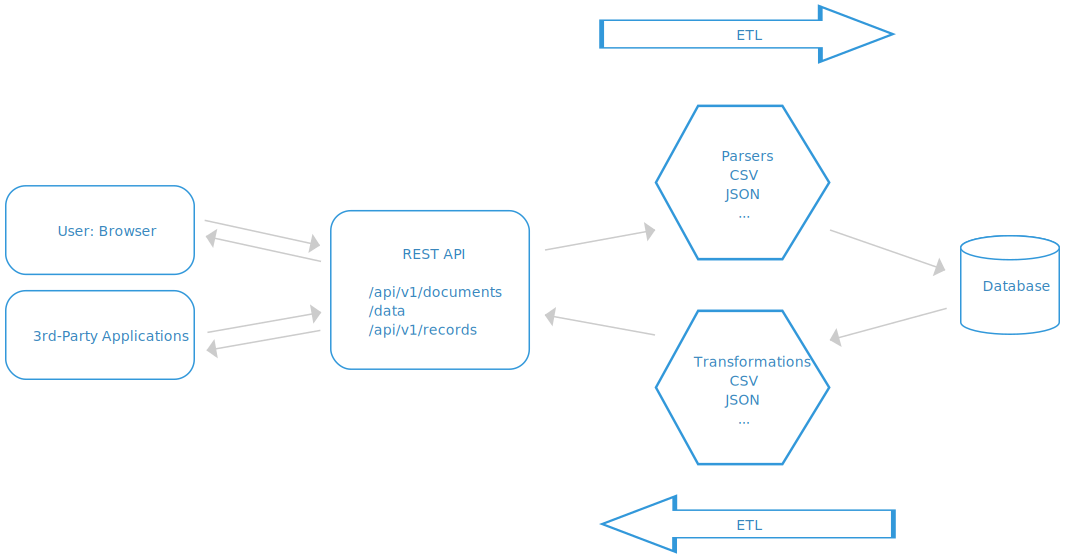
\includegraphics[width=\linewidth]{../projektdokumentation/fig/ODH-Architecture-Overview}
    \caption{Grobe Architektur-Übersicht}
    \label{fig:tb:arch-overview}
\end{figure}

\subsection{Internes Format}
Es wurden diverse Optionen sowohl zur Speicherung wie auch zur Transformation der Daten in Betracht gezogen und im Hinblick auf deren Vor- und Nachteile bezüglich Machbarkeit, Komplexität und Performance evaluiert. Die Daten werden von Parser-Modulen in sogenannte DataFrame Objekte geladen. Ein DataFrame ist ein Tabellen-artiges Objekt der Pandas\footnote{\url{http://pandas.pydata.org/}} Python-Bibliothek. Pandas ist eine mächtige ``Data-Analysis'' Bibliothek, welche aufgrund der zugrundeliegenden NumPy\footnote{\url{http://www.numpy.org/}} Bibliothek sehr effizient ist.
Zu jedem Format kann auch ein Formatter-Modul implementiert werden, welches hingegen ein DataFrame entgegennimmt und einen Output des gewünschten Formates zurückgibt.

\subsection{Schema-Transformation}
Auch bei der Homogenisierung des Schemas wurden diverse Möglichkeiten, welche teilweise eng mit dem Format gekoppelt\footnote{Die Persistierung der Daten in eines Postgres Datenbank impliziert beispielsweise die Verwendung von PostgreSQL zur Transformation} sind analysiert. Schlussendlich wurde eine eigene \gls{dsl} implementiert \textendash\ die \acf{odhql}. \acs{odhql} ist eine an \acs{sql} angelehnte \gls{dsl} inklusive Unterstützung einiger Geo-Basisfunktionalität analog der PostGIS Erweiterung von PostgreSQL.

\subsection{Erweiterbarkeit}
Sowohl die Unterstützung von Dateiformaten\footnote{CSV, KML, Excel, \dots} wie auch die vorhandenen Funktionen der \acf{odhql} wurden mit Bedacht auf Erweiterbarkeit implementiert. Eine Drittpartei kann durch Implementation eines speziellen Interfaces eigene Parser/Formatter Paare oder gar \gls{odhql} Funktionen zur Verfügung stellen, welche nach einem Neustart der Applikation sofort verfügbar sind.


\chapter{Resultate und Ausblick} \label{sec:tb:results}
Mit Ausnahme der Unterstützung von GeoPackage wurden alle in der Aufgabenstellung gestellten Ziele erreicht. Der Grund für die mangelnde GeoPackage-Unterstützung ist eine Serie von Fehlern in GDAL (siehe \cref{sec:pd:format-gdal-problems}).

\begin{figure}[H]
    \centering
    \includegraphics[width=2\linewidth/3]{fig/odh-package-list}
    \caption{ODH: Paket-Liste}
\end{figure}

Ein Benutzer kann bereits vorhandene Daten durchsuchen und herunterladen. 

\begin{figure}[H]
    \centering
    \includegraphics[width=2\linewidth/3]{fig/odh-document-detail}
    \caption{ODH: Detail zu hochgeladenen Daten}
\end{figure}

Daten können als Datei oder Gruppe von Dateien hochgeladen oder von einer URL bezogen werden.

\begin{figure}[H]
    \centering
    \includegraphics[width=2\linewidth/3]{fig/odh-offer-data}
    \caption{ODH: Daten anbieten}
\end{figure}

Die Resultate von Transformationen präsentieren sich ähnlich wie hochgeladene Dateien.

\begin{figure}[H]
    \centering
    \includegraphics[width=2\linewidth/3]{fig/odh-transformation-detail}
    \caption{ODH: Details einer Transformation (1)}
\end{figure}

Mit minimaler Einführung können einfache Transformationen zusammengeklickt werden, mit ODHQL-Kenntnissen können auch komplexe Transformationen geschrieben werden. Als Datenquellen dienen hochgeladene Daten, \acs{wfs}-Server oder bereits bestehende Transformationen.

\begin{figure}[H]
    \centering
    \includegraphics[width=2\linewidth/3]{fig/odh-transformation-assistant}
    \caption{ODH: Transformations-Assistent}
\end{figure}

Bereits vorhandene Transformationen können geklont, oder bei eigenen Transformationen auch bearbeitet werden.

\begin{figure}[H]
    \centering
    \includegraphics[width=2\linewidth/3]{fig/odh-edit-transformation}
    \caption{ODH: Details einer Transformation (2)}
\end{figure}

\section{Persönlicher Bericht}

\subsection{Christoph Hüsler}
Meine Python-Vorkenntnisse waren relativ beschränkt - ich kannte die Syntax von Code-Beispielen, die mir über die Jahre im Internet begegnet sind und ich hatte bereits ein paar kleinere Skripts angepasst, aber nie ein eigenens Projekt mit Python realisiert. Trotzdem gelang es mir schnell, mich einzuarbeiten.

Highlight dieser Arbeit war für mich sicher die Implementation des ODHQL-Parsers mit pyparsing - ich kann dieses Modul nur empfehlen. 

Auch die Zusammenarbeit im Team empfand ich als sehr positiv. Trotz einiger Differenzen konnten wir immer miteinander diskutieren und eine Lösung finden. 

\subsection{Remo Liebi}
\xxx rliebi

\subsection{Fabio Scala}
\xxx fscala


\section{Dank}
In erster Linie möchten wir uns bei unserem Betreuer, \proff, für die Unterstützung während der gesamten Laufzeit der Arbeit bedanken. Zudem gilt auch Herrn Dorfschmid von Adasys AG ein besonderer Dank für das konstruktive Gespräch und die architektonische Inspiration für OpenDataHub. 

An dieser Stelle möchten wir uns auch bei Herrn Kalberer, Entwickler von ogrtools und INTERLIS Treiber für GDAL sowie der GDAL Community für die stets rasche Rückmeldung auf Fehlerberichte unsererseits bedanken.
